%        File: manual.tex
%     Created: Thu May 23 08:00 AM 2019 E
%
\documentclass[letterpaper,11pt]{article}
\usepackage[leqno]{amsmath}
\usepackage{mathptmx,courier}
\usepackage[scaled]{helvet}
\usepackage[inter-unit-product=\ensuremath{{}\cdot{}},per-mode=symbol,separate-uncertainty,binary-units]{siunitx}
\usepackage[nohead,letterpaper,lmargin=0.75in,rmargin=0.75in,tmargin=0.75in,bmargin=0.75in]{geometry}
\usepackage{paralist}
\usepackage[pdftex]{graphicx}
\usepackage[hyperfigures=false,bookmarks=false,pdftex,colorlinks,linkcolor=black,urlcolor=blue]{hyperref}
\usepackage{fancyhdr,pageslts}
\usepackage[cachedir=/home/kjh016/tmp/mintedcache]{minted}
\usepackage{fancyvrb}
\newcommand\userinput[1]{\textbf{#1}}
\usepackage{tcolorbox}

\graphicspath{{graphics/}}

\ifpdf\pdfinfo{
  /Title (Firefly Simulator User's Manual) %FIXME
  /Author (K. J. Hass, Bucknell University) %FIXME
/Keywords () }
\fi

\pagestyle{fancy}
\fancyhf{}
\fancyfoot[C]{Page \thepage\ of \pageref*{LastPage}}
\fancyfoot[R]{Revised \today}
\fancyfoot[L]{\includegraphics[height=12pt]{CC_BY_SA_NC_sml}\ K. Joseph Hass}
\pagenumbering{arabic}  % required by pageslts
\renewcommand\headrulewidth{0pt}

\begin{document}
\Large
\centerline{Firefly Simulator User's Manual}
\normalsize
\subsection*{Introduction}

The \textit{firefly simulator} is a device that is used to illuminate
light-emitting diodes (LEDs) in order to simulate the flashing of fireflies.
The simulator allows the user to program (or \textit{configure}) the
brightness, duration, and other aspects of the LED flashes so that a wide
variety of different kinds of flashes can be created. The heart of the firefly
simulator is an Arduino microcontroller.

The simulated firefly behavior is described in terms of \textit{LEDs},
\textit{channels}, \textit{flashes}, \textit{patterns}, and \textit{random
pattern sets}. Each of these terms
has a very specific meaning in this context. When using the simulator, true
physical LEDs are connected by cables to the output channels of the simulator.
Each channel corresponds to a numbered electrical connector on the side of
the simulator enclosure. Within the simulator software a set of
\textit{virtual LEDs} can be defined, where a virtual LED consists of a
specified channel and a specified maximum brightness level.

A virtual LED is then used to define a \textit{flash}. A flash definition
includes the choice of a specific virtual LED as well as the timing parameters
that determine how quickly the LED changes from completely dark to fully
illuminated, how long the LED stays fully illuminated, how quickly the LED
changes to completely dark, and how long the LED must remain dark before
another flash can begin.

One or more flashes can then be combined into a \textit{pattern}. The flashes
associated with a particular pattern are executed first, in the specified
order, and then all LEDs are kept dark until the specified duration of the
pattern ends. 

Multiple patterns can be combined into a \textit{random pattern set}. As the
name suggests, the patterns specified in a random pattern set can be executed
continuously in a random order.

The simulator is initially configured using a USB connection to a host
computer. However, all configuration information is stored in nonvolatile
memory within the simulator and a small keypad on the simulator itself can
be used to execute flashing patterns. Thus, the simulator can be made portable
and used in the field without a host computer.

\subsection*{Connections}
\subsubsection*{Power/USB}

A single USB connector on the simulator is used to supply power to the device
as well as to support the interface with the host computer. The computer
interface is actually an asynchronous serial interface that is emulated via
USB. A description of the interface parameters and communication protocol is
provided below.

\subsubsection*{Physical LEDs}

A \textit{physical LED} consists of a small circuit board connected to a cable
that can be connected to the simulator. An actual LED is mounted on the circuit
board, as well as other components that are used to regulate and limit the
electrical current through the LED.

Up to six physical LEDs can be simultaneously connected to the simulator, by
plugging their cables into the six \textit{LED channel} connectors on the side
of the simulator.

It is the user's responsibility to mark each physical LED with a unique
identifier and maintain records of the optical characteristics of that LED.
It is also the user's responsibility to track which physical LED is connected
to each LED channel.

\subsubsection*{Abort Button}

The \textit{abort button} is a red pushbutton located on the top of the
simulator enclosure. Pressing this button will cause the simulator to be reset
to its initial state, the same state that it is in when power is first applied.
Some of the commands described below will cause the simulator to execute
flashes continuously, and in that case pressing the abort button is necessary
to halt the simulator. 

\subsection*{Communications}

The firefly simulator communicates with a host computer using a serial
communications interface, which is called a \texttt{COM} port in Windows or a
\texttt{/dev/tty} in Linux and MacOS. This interface can be used to configure
the simulator and to log its operation.

The simulator has been programmed to operate at 9600 baud with 8 data bits,
no parity, 1 stop bit, and no flow control.

The user can send commands to the simulator using a terminal simulator program
on the host computer, and the simulator's responses will also appear on the
terminal. The command messages sent by the host computer are simple strings of
text. Each command begins with one or two \textbf{capital} letters, followed
by some number of \textbf{fields} or \textbf{parameters} for the command. The
different fields of a message are separated by a \textbf{comma}. Each command
must be terminated with a carriage return and/or linefeed, which are typically
added just by pressing the ``\texttt{Enter}'' key.

\subsection*{Virtual LEDs}

The simulator software has no information about what, if any, physical LEDs are
connected to its LED channels. Instead, the simulator software is configured to
control \textit{virtual LEDs}. A virtual LED is defined by assigning to it a
physical LED channel number as well as a maximum brightness value (0 to 100).
Note that the maximum brightness level is treated as a percentage of the
maximum current available to the physical LED. For example, if a particular
physical LED circuit board has been designed to limit the LED current to
\SI{20}{\milli\ampere}, and then setting the maximum brightness of a virtual
LED to \texttt{50}, will result in an average LED current of
\SI{10}{\milli\ampere} when the LED is ``on''.

Each virtual LED has a unique \textit{LED number}, which is simply an integer
used to identify a particular virtual LED so it can be used later. The
simulator can typically store up to 16 distinct virtual LED definitions.

Note that a given LED channel (i.e.\ a given physical LED) can be used in more
than one virtual LED definition. This allows the same physical LED to be used
at different brightness levels.

The command message used to configure a virtual LED begins with the letter `L'
and has three fields: the virtual LED number, the LED channel number, and the
maximum brightness level. The fields must be integer values. For example, the
commands shown here will first configure virtual LED \#7 to use the physical
LED on channel 3 with a maximum brightness equivalent to 80\% of its maximum
possible current. Virtual LED \#1 is then configured to use channel 2 with
100\% of its maximum current. If the format of the command is correct and the
fields have appropriate values, then the simulator will respond with
``\texttt{LED Configured}''.  (For the examples shown in this document, the
text typed by the user is shown in a bold typewriter font and the simulator's
response is shown in a normal typewriter font. Note that all human-readable
messages issued by the firefly simulator are subject to change with future
versions of the simulator software.)

\begin{tcolorbox}
\begin{Verbatim}[commandchars=\\\{\}]
\userinput{L,7,3,80}
LED Configured
\userinput{L,1,2,100}
LED Configured
\end{Verbatim}
\end{tcolorbox}

Note that once configured a virtual LED can be modified simply by rewriting
its definition. Defining the same virtual LED number multiple times does not
produce an error but only the last definition will be saved.
The LED configuration command will fail if
\begin{compactitem}
  \item the LED number is out of range (1 to 16 for an Arduino UNO), or
  \item the channel number is invalid (1 to 6 for an Arduino UNO), or
  \item the maximum brightness is zero, or
  \item the maximum brightness is greater than 100
\end{compactitem}

The \texttt{DL} (Dump LEDs) command will list all of the virtual LEDs that
have been configured in the simulator. There are no additional fields for this
command. Note that each virtual LED is listed using the same format as the
command used to configure it, except that the first letter is a lower-case
`l'.
\begin{tcolorbox}
\begin{Verbatim}[commandchars=\\\{\}]
\userinput{DL}
Saved LEDs
l,1,2,100
l,7,3,80
\end{Verbatim}
\end{tcolorbox}

The \texttt{XL} (eXecute LED) command can be used to manually turn an LED on
or off. This command has two fields: the virtual LED number and the desired
brightness level. The brightness level must be from 0 to 100, and is a
percentage of the maximum LED current. The commands shown below will turn
on virtual LED \#1 at 100\% of its possible brightness, and then turn it off.
\begin{tcolorbox}
\begin{Verbatim}[commandchars=\\\{\}]
\userinput{XL,1,100}
Executing LED 1
\userinput{XL,1,0}
Executing LED 1
\end{Verbatim}
\end{tcolorbox}

\subsection*{Flashes}

A \textit{flash} is the process of illuminating a given virtual LED for a
given amount of time. In addition, the parameters of a flash specify a time
interval from when the LED becomes dark until another flash can occur.

The timing parameters of a flash are shown in Fig.\ \ref{fig:FlashPulse}.
At the beginning of a flash the illumination level of the LED may be
increased linearly over a period of time, called the \textit{up duration},
until the LED is fully illuminated at its maximum brightness level. Similarly,
after the LED is kept at full illumination for its \textit{on duration}, the
illumination level may be linearly decreased over a period of time called
the \textit{down duration}. The total duration of a flash is its
\textit{interpulse interval}. If the sum of the up duration, on duration, and
down duration is less than the interpulse interval then the LED will remain
dark until the full interpulse interval time has elapsed.

\begin{figure}[h]
  \begin{center}
    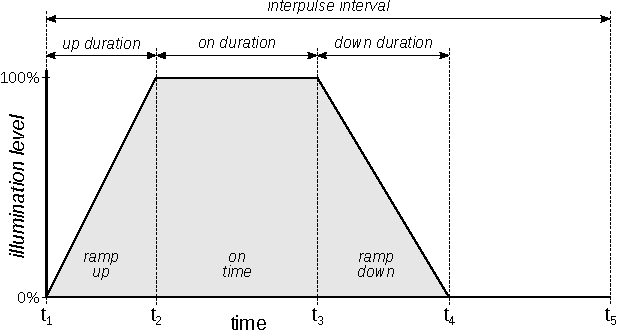
\includegraphics{Flashes_FlashPulse}
  \end{center}
  \vspace{-18pt}
  \caption{\textit{flash} waveform}
  \label{fig:FlashPulse}
\end{figure}

The command message used to configure a flash begins with the letter `F'
and has six fields: the flash number, the virtual LED number, the up
duration, the on duration, the down duration, and the interpulse interval.
The fields must be non-negative integer values. All duration and interval times
are specified in milliseconds; the up duration and down duration should be
multiples of \SI{10}{\ms}.

For example, the commands shown below will configure flash \#4
to use virtual LED \#3. The LED's illumination will ramp up from fully dark to
its maximum brightness in \SI{200}{\ms}, stay at maximum brightness
for \SI{300}{\ms}, and then ramp down from maximum brightness to fully
dark over \SI{400}{\ms}. The interpulse interval is specified as
\SI{1.2}{\second}, and the LED is partially or fully illuminated for a total of
\SI{900}{\ms}, so the LED will remain dark for an additional
\SI{600}{\ms} before the next flash can begin.

\begin{tcolorbox}
\begin{Verbatim}[commandchars=\\\{\}]
\userinput{F,4,3,200,300,400,1500}
Flash Configured
\end{Verbatim}
\end{tcolorbox}

Attempting to configure a flash number that is already configured will cause
the new definition to replace the existing definition, without warning.
If the format of the command is correct and the fields have appropriate values,
then the simulator will respond with ``\texttt{Flash Configured}''. The command
will fail if
\begin{compactitem}
  \item the flash number or LED number is out of range (1 to 16 for the
    Arduino UNO), or
  \item the up duration, on duration, or down duration is greater than
    \SI{32.767}{\ms}, or
  \item the interpulse interval is zero, or
  \item the interpulse interval is less than the sum of the up duration, on
    duration, and down duration.
\end{compactitem}

The \texttt{DF} (Dump Flashes) command will list all of the flashes that
have been configured in the simulator. There are no additional fields for this
command. All configured flashes are listed, in numerical order. Note that flash
\#3 has not yet been configured in this example.

\begin{tcolorbox}
\begin{Verbatim}[commandchars=\\\{\}]
\userinput{DF}
f,1,1,120,500,150,2000
f,2,2,200,200,200,1000
f,4,3,200,300,400,1500
f,5,6,200,300,400,1200
\end{Verbatim}
\end{tcolorbox}

The \texttt{XF} (eXecute Flash) command can be used to execute a specific
flash.  This command has one field, the flash number. The specified flash
will be executed repeatedly and the simulator will not accept any further
commands. The \textsf{ABORT} button must be pressed to terminate this command.

\begin{tcolorbox}
\begin{Verbatim}[commandchars=\\\{\}]
\userinput{XF,4}
Executing flash number 4
\end{Verbatim}
\end{tcolorbox}

\subsection*{Patterns}

A \textit{pattern} is the process of executing one or more flashes in a
given amount of time. The set of flashes to be executed is called the
\textit{flash list}, which may contain up to 16 flash numbers. The flash
numbers in the pattern can all be unique, or a given flash number may be
repeated. In addition, the parameters of a pattern specify a time interval
from when the last flash ends until another pattern can begin (the
\textit{flash pattern interval}).

The timing parameters of an example pattern are shown in
Fig.\ \ref{fig:FlashPattern}. For this example the sum of the interpulse
intervals of the four flashes in the pattern is \SI{6.7}{\second}, and the
flash pattern interval is specified as \SI{10}{\second}, so all of the LEDs are
kept dark for an additional \SI{3.3}{\second} after the fourth flash (that is,
the second occurrence of flash \#1) ends.

\begin{figure}[h]
  \begin{center}
    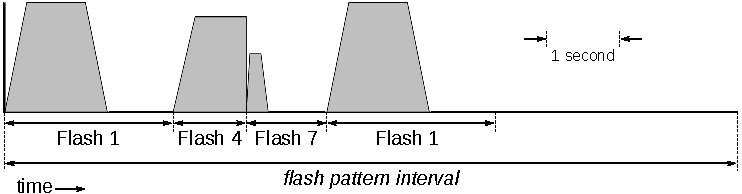
\includegraphics{Flashes_PatternTimeline2}
  \end{center}
  \vspace{-18pt}
  \caption{\textit{pattern} timeline}
  \label{fig:FlashPattern}
\end{figure}

The commands shown below could be used to completely configure the pattern
shown in Fig.\ \ref{fig:FlashPattern}. Assume that the same physical LED is
used for all of the flashes, and that this LED is connected to channel 5. Three
virtual LEDs are first defined, all of which use the same channel but have
different maximum brightness levels (53\% for flash \#7, 87\% for flash \#4,
and 100\% for flash \#1, respectively).
Then the three flashes are defined with the desired timing parameters. Note
that flash \#4 has a value of zero for its down duration, so the LED instantly
changes from full illumination to fully dark. The interpulse interval for flash
\#3 is also exactly equal to the up duration plus the on duration, so the next
flash can begin immediately after the LED is turned off.

The pattern itself is defined using the `P' command. This command has a minimum
of three fields: the pattern number, the flash pattern interval, and the flash
number of a single flash that will be executed in the pattern. Additional
members of the flash list are appended as comma-separated values, so the
command may have a total of 18 fields if a list of 16 flashes is included in
the pattern. The command shown in this example configures pattern \#2 to have
a flash pattern interval of \SI{10}{\second} and to begin by executing flashes
\#1, \#4, \#7, and \#1.

\begin{tcolorbox}
\begin{Verbatim}[commandchars=\\\{\}]
\userinput{L,1,5,53}
LED Configured
\userinput{L,2,5,87}
LED Configured
\userinput{L,3,5,100}
LED Configured
\userinput{F,1,3,300,800,300,2300}
Flash Configured
\userinput{F,4,2,300,700,0,1000}
Flash Configured
\userinput{F,7,1,50,150,100,1100}
Flash Configured
\userinput{P,2,10000,1,4,7,1}
Pattern Configured
\end{Verbatim}
\end{tcolorbox}

Attempting to configure a pattern number that is already configured will cause
the new definition to replace the existing definition, without warning.
The pattern configuration command will fail if
\begin{compactitem}
  \item the pattern number is out of range (1 to 16 for the Arduino UNO), or
  \item any of flashes given in the flash list has not been configured, or
  \item the flash pattern interval is greater than \SI{32.767}{\ms}, or
  \item the flash pattern interval is zero, or
  \item the flash pattern interval is less than the sum of the interpulse
    intervals for the flashes in the flash list.
\end{compactitem}

The \texttt{DP} (Dump Patterns) command will list all of the patterns that
have been configured in the simulator. There are no additional fields for this
command. All configured patterns are listed, in numerical order. Note that
pattern \#4 has not yet been configured in this example.

\begin{tcolorbox}
\begin{Verbatim}[commandchars=\\\{\}]
\userinput{DP}
p,1,7500,1,2,3
p,2,10000,1,4,7,1
p,3,5000,3,3
p,5,32100,16
\end{Verbatim}
\end{tcolorbox}

The \texttt{XP} (eXecute Pattern) command can be used to execute a single
specific pattern.  This command has one field, the pattern number.
The specified pattern will be executed repeatedly and the simulator will
not accept any further commands; the \textsf{ABORT} button must be pressed
to terminate this command.  The simulator sends a message back to the host
computer before beginning each execution of the selected pattern. This
response message begins with the letter `p' and has three additional fields:
the current data and time (UTC), the current Celsius temperature, and the
pattern number for the pattern that is about to begin.

\begin{tcolorbox}
\begin{Verbatim}[commandchars=\\\{\}]
\userinput{XP,2}
p,2019-05-29T18:12:44Z,22,2
p,2019-05-29T18:12:54Z,22,2
p,2019-05-29T18:13:04Z,23,2
p,2019-05-29T18:13:14Z,22,2
  \textit{and so on\dots}
\end{Verbatim}
\end{tcolorbox}

\subsection*{Random Pattern Sets}

A \textit{random pattern set} is simply a set, or list, of unique pattern
numbers. The firefly simulator will repeatedly execute these patterns, using
a pseudorandom number generator to select the next pattern to be executed

The command message used to configure a random pattern set begins with the
letter `R' and has a minimum of 2 fields: the random pattern set number and
the pattern number for a single pattern to be executed. However, a random
pattern set with a single pattern will behave exactly like an \texttt{XP}
(eXecute Pattern) command that specifies the single pattern. A practical random
pattern set command will have up to 17 fields: the random pattern set number
and up to 16 pattern numbers. Note that the order that the pattern numbers are
given in the pattern set is not significant, but a given number must not be
repeated.

For example, the command shown below will configure random pattern set \#4,
which will randomly execute patterns \#1, \#2, and \#5.
\begin{tcolorbox}
\begin{Verbatim}[commandchars=\\\{\}]
\userinput{R,4,1,2,5}
Random Pattern Set Configured
\end{Verbatim}
\end{tcolorbox}

Attempting to configure a random pattern set number that is already configured
will cause the new definition to replace the existing definition, without
warning. The random pattern set configuration command will fail if
\begin{compactitem}
  \item the random pattern set number is out of range (1 to 16 for an Arduino
    UNO), or
  \item any of patterns given in the pattern list has not been configured.
\end{compactitem}

The \texttt{DR} (Dump Random pattern sets) command will list all of the random
pattern sets that have been configured. This command has no parameters.
\begin{tcolorbox}
\begin{Verbatim}[commandchars=\\\{\}]
\userinput{DR}
r,2,3,5,13
r,3,1,2,3,4
r,4,1,2,5
\end{Verbatim}
\end{tcolorbox}

The \texttt{XR} (eXecute Random pattern set) command can be used to execute a
specific random pattern set. This command has one field, the random pattern set
number. The patterns specified in the random pattern set will chosen at random
and executed repeatedly until the \textsf{ABORT} button is pressed. The
simulator sends a message back to the host computer before beginning each
execution of a selected pattern. This response message begins with the letter
`p' and has three additional fields: the current data and time (UTC), the
current Celsius temperature, and the pattern number for the pattern that
is about to begin.

\begin{tcolorbox}
\begin{Verbatim}[commandchars=\\\{\}]
\userinput{XR,4}
Generating Random Patterns
r,4,1,2,5
p,2019-05-30T15:33:26Z,23,5
p,2019-05-30T15:33:59Z,22,1
p,2019-05-30T15:34:06Z,22,2
p,2019-05-30T15:34:16Z,22,5
p,2019-05-30T15:34:49Z,22,1
  \textit{and so on\dots}
\end{Verbatim}
\end{tcolorbox}

\subsection*{Using the Keypad}

The firefly simulator's built-in keyboard can be used to execute a single
pattern repeatedly or to execute a random pattern set. Pressing the asterisk
`*' key followed by a digit key from 1 to 9 has exactly the same effect as
entering the \texttt{XP,}\textit{n} command from the host computer, where
\textit{n} is the digit key that was pressed. Similarly, pressing the number
sign `\#' key followed by a digit key from 1 to 9 has exactly the same effect
as entering the \texttt{XR,}\textit{n} command.

\end{document}


